% QuantImmuBench — benchmark × position paper
% 主投 Briefings in Bioinformatics（OUP）。先用通用 article 类成稿，投稿前换 oup-authoring-template。
% 双盲：0 个人/机构/导师/HPC 名。数字只用已核 csv，DTU 工具标 pending DTU consent。
\documentclass[11pt]{article}

\usepackage[utf8]{inputenc}
\usepackage[T1]{fontenc}
\usepackage{geometry}
\geometry{margin=1in}
\usepackage{graphicx}
\usepackage{booktabs}
\usepackage{amsmath}
\usepackage{amssymb}
\usepackage{multirow}
\usepackage{xcolor}
\usepackage{hyperref}
\hypersetup{colorlinks=true, linkcolor=blue, citecolor=blue, urlcolor=blue}
\usepackage[numbers,sort&compress]{natbib}
\usepackage{siunitx}

% \todo 占位（投前必清零）
\newcommand{\todo}[1]{\textcolor{red}{\textbf{[TODO: #1]}}}
% pending DTU 标记
\newcommand{\pendingDTU}{\textcolor{orange}{$^{\dagger}$}}

\title{\textbf{Existing Neoantigen Immunogenicity Predictors Do Not Quantify
T-Cell Response Magnitude: A Benchmark and the Case for Per-Patient Evaluation}}

\author{Anonymous (double-blind submission)}
\date{}

\begin{document}
\maketitle

\begin{abstract}
\noindent\textbf{Motivation.} Personalized neoantigen vaccines depend on
selecting, from many candidate mutations, the few that will provoke a strong
T-cell response. A large family of immunogenicity predictors now decides whether
a peptide is recognized at all, but \emph{how strong} the response will
be---its magnitude---is essentially unaddressed, even though graded experimental
readouts such as ELISpot spot-forming counts make this quantity measurable. It is
not known how well existing tools track response magnitude when their scores are
repurposed as continuous predictors, nor whether the apparent differences between
them are real.

\noindent\textbf{Results.} We assemble a unified benchmark that places eight
immunogenicity tools and one presentation proxy on a common footing through a
seven-step harmonization protocol, and scores them against a continuous ELISpot
magnitude readout as well as a binary recognition label on a common patient
cohort (DS2, $101$ peptides). Three findings emerge. First, the correlation with
response magnitude is uniformly weak: every tool falls below an absolute Spearman
correlation of $0.33$, and binary-discrimination differences, while larger in
point estimate, have broadly overlapping bootstrap intervals that shift with
aggregation and threshold, so no single tool is statistically distinguishable as
best at the top of the panel. Second, a per-patient evaluation
protocol---correlating within each patient before aggregating---surfaces
within-patient ranking ability in a subset of patients that the default global
metric conceals, together with large individual variation. Third, we quantify
the magnitude gap and argue, with an explicit biological ceiling, that it is an
open opportunity rather than a closed problem.

\noindent\textbf{Conclusion.} Response magnitude remains an unfilled gap with a
genuine biological upper bound; our reproducible benchmark and per-patient
protocol provide a measuring stick for the continuous-magnitude predictors that
this gap invites.

\end{abstract}

\noindent\textbf{Keywords:} neoantigen; immunogenicity prediction; T-cell response magnitude;
benchmark; ELISpot; per-patient evaluation; cancer vaccine.

\section{Introduction}
\label{sec:intro}

Personalized neoantigen vaccines have moved from concept to the clinic, with
early-phase trials reporting durable, mutation-specific T-cell responses and
encouraging signals of clinical benefit across several tumour types
\cite{Sahin2023,NatRevImmunol2023}. Their central computational bottleneck is
selection: from the hundreds of somatic mutations in a tumour, only a handful of
mutated peptides will actually be recognized by a patient's T cells, and only a
fraction of those will mount a response strong enough to matter clinically.
Decades of work have made it clear that peptide--MHC binding, while necessary, is
far from sufficient for immunogenicity. The TESLA consortium benchmark made this
gap quantitative: of the strongly presented candidate peptides nominated across
participating teams, only on the order of six percent proved experimentally
immunogenic \cite{TESLA2020}. Prioritizing neoantigens for a vaccine therefore
demands predictors that reach beyond binding into the immunological consequences
of presentation.

The literature has approached this problem along what is best described as a
capability ladder. At the first level (L1), binding predictors such as
NetMHCpan and MHCflurry estimate peptide--MHC affinity or eluted-ligand
likelihood across thousands of alleles \cite{NetMHCpan2020,MHCflurry2020}. At
the second level (L2), presentation-aware models such as PRIME and BigMHC
incorporate mass-spectrometry eluted-ligand evidence to estimate the probability
that a peptide is genuinely presented \cite{PRIME2023,BigMHC2023}. At the third
level (L3), a large and architecturally diverse family of immunogenicity tools
asks the binary question of whether a presented peptide will be recognized by T
cells at all
\cite{DeepImmuno2021,deepHLApan2019,IMPROVE2024,PredIG2025,ICERFIRE2024,NeoaPred2024,ImmunoStruct2025,NetTepi2014,Seq2Neo2022,TSCAPE2025,CNNeoPP2026}.
A fourth concern, the \emph{magnitude} of the elicited response---how strong the
T-cell reaction is, rather than merely whether it occurs---remains essentially
unaddressed. We stress that this fourth concern is not a strictly higher rung of
the same ladder. Levels L1 through L3 sharpen a single binary judgement, whereas
magnitude is a \emph{regression axis orthogonal} to that judgement: one can ask
how strong a response will be at the presentation layer just as well as at the
recognition layer. We therefore treat magnitude (L4) as an orthogonal
quantitative dimension layered across the binary ladder, not as a successor to
it.

This orthogonal magnitude dimension is the gap that motivates our study.
Surveying more than a dozen immunogenicity methods published between 2024 and
2026, together with six recent reviews, we find that no tool is explicitly
designed to regress the continuous magnitude of the T-cell response and report
correlation or error against a continuous experimental readout; every method
ultimately emits a binary call or a binding-strength score
\cite{explorationpub2023,Zhao2025,BiomarkerRes2025}. The gap is striking
precisely because the signal is often available and then discarded: PredIG is
trained on data carrying graded positive-low, intermediate, and high labels that
are binarized before use \cite{PredIG2025}; ICERFIRE explicitly collapses graded
labels into a single class \cite{ICERFIRE2024}; and CNNeoPP's validation ELISpot
data distinguish weak from strong responders yet the model still outputs only a
binary decision \cite{CNNeoPP2026}. That a gap has gone unfilled, however, is not
by itself evidence that filling it is worthwhile. An absence in the literature
admits two readings: an open opportunity, or a problem that practitioners have
quietly judged intractable. Sequence-level magnitude prediction has a genuine
biological ceiling---the magnitude of a polyclonal T-cell response depends
heavily on donor-specific precursor frequencies that no peptide-and-allele input
can observe, plausibly capping the explainable variance at a Spearman
correlation of roughly $0.4$ to $0.6$. We take this ceiling seriously throughout,
and frame the value of continuous prediction not as high-precision regression but
as recovering ranking-relevant signal for clinical top-$K$ prioritization that
binary tools throw away.

Before a new magnitude predictor can be justified, however, a prior question must
be answered empirically: how well do today's tools actually track response
magnitude when their scores are repurposed as continuous predictors, and are the
apparent differences between them real? This question has not been asked under a
controlled, apples-to-apples protocol, in part because immunogenicity tools
differ in input formats, allele handling, score scales, and aggregation
conventions, so that head-to-head numbers are rarely comparable across papers. We
close this gap with a unified benchmark. Using a common ELISpot ground truth and
a seven-step harmonization protocol that standardizes inputs, alleles, and
scoring across tools, we evaluate eight immunogenicity tools and one presentation
proxy against the continuous ELISpot spot-forming-cell readout, and against the
binary positive/negative outcome, on a common patient cohort.

Our findings and contributions are threefold.
\textbf{First}, under this harmonized protocol the correlation between existing
tool scores and ELISpot magnitude is uniformly weak or non-significant: all tools
fall below an absolute Spearman correlation of $0.33$, with only IMPROVE and
PredIG reaching significance under particular aggregation choices, and the
binary-discrimination performance, while higher in point estimate, has bootstrap
confidence intervals that overlap so broadly---and shift so much with aggregation
and threshold choices---that no single tool can be declared best. A presentation
proxy performs near chance on magnitude, reinforcing that presentation,
immunogenicity, and response magnitude are distinct quantities. \textbf{Second},
we show that the global correlation metric used by default in the field masks
substantial individual variation, and we introduce a per-patient evaluation
protocol---computing a correlation within each patient and then aggregating---that
exposes it: tools whose pooled global correlation is indistinguishable from noise
recover meaningful within-patient ranking ability, while across-patient spread is
large. This aligns benchmark evaluation with the cohort-level paradigm of the
clinical literature \cite{TESLA2020,Muller2023}. \textbf{Third}, we quantify the
magnitude gap and synthesize the evidence that the field has systematically set
it aside, providing a reproducible benchmark and protocol that any future
continuous-magnitude predictor can be measured against, while being explicit
about the biological ceiling that bounds what such a predictor can achieve.

\section{Background and Related Work}
\label{sec:related}

We organize the related work around the capability ladder introduced above,
tracing the progression from binding through presentation to binary
immunogenicity, and then situating the orthogonal magnitude dimension that our
benchmark targets. We also explicitly delimit a set of tools that produce
continuous outputs but along axes distinct from response magnitude, since these
are the most likely to be mistaken for existing magnitude predictors.

\subsection{The neoantigen prediction ladder}
\label{sec:related:ladder}

Computational prediction of tumour neoantigens has progressed along a capability
ladder: from peptide--MHC binding affinity, to antigen presentation, to binary
T-cell immunogenicity, and---only nominally---to the magnitude of the elicited
T-cell response. Recent surveys frame the discovery pipeline as a sequence of
stages running from HLA typing and variant calling through pMHC presentation to
pMHC recognition \cite{Zhao2025,BiomarkerRes2025}. A recurring lesson across this
literature is that MHC binding is necessary but not sufficient for
immunogenicity: in the TESLA consortium benchmark, only on the order of six
percent of strongly presented candidate peptides were experimentally
immunogenic \cite{TESLA2020}. We emphasize that this ladder describes a
stratification of prediction \emph{targets} rather than a partition of tools into
mutually exclusive bins; modern tools routinely span levels, with binding
predictors emitting both affinity and eluted-ligand scores and immunogenicity
models consuming presentation percentiles as input features.

\subsection{From binding to presentation (L1--L2)}
\label{sec:related:binding}

Binding predictors such as NetMHCpan-4.1 \cite{NetMHCpan2020} and MHCflurry~2.0
\cite{MHCflurry2020} estimate peptide--MHC affinity or eluted-ligand presentation
across thousands of alleles. Presentation-aware models, including PRIME
\cite{PRIME2023} and the eluted-ligand variant of BigMHC \cite{BigMHC2023},
integrate mass-spectrometry eluted-ligand data to estimate the probability that a
peptide is genuinely presented. It is important to recognize that these
continuous outputs quantify binding strength or presentation likelihood, not
response magnitude: the affinity scale is a different physical dimension from the
intensity of a polyclonal T-cell response, and benchmark studies report only weak
correlation between binding scores and ELISpot magnitude
\cite{explorationpub2023,Buckley2022}.

This distinction matters because several established tools produce continuous
scores and could be misread as pre-existing quantitative magnitude predictors.
Three classes warrant explicit delimitation. First, binding-affinity predictors
report a continuous affinity in nanomolar units or a percentile rank
\cite{NetMHCpan2020,MHCflurry2020}. Second, stability predictors such as
NetMHCstabpan estimate a continuous peptide--MHC complex half-life
\cite{NetMHCstabpan2016}. Third, TCR--pMHC models such as pMTnet output a
continuous recognition ranking percentile \cite{pMTnet2021}. None of these
targets the quantity of interest here. Each is continuous along a dimension---
binding affinity, complex stability, or TCR--pMHC recognition propensity---whose
units are not those of a population-level T-cell response measured in
spot-forming cells, and each correlates only weakly with ELISpot magnitude. We
therefore treat these continuous neighbours not as magnitude predictors but as
natural control baselines against which any genuine magnitude regression should
be compared.

\subsection{Immunogenicity classification (L3)}
\label{sec:related:immuno}

The bulk of neoantigen immunogenicity tools target a binary outcome---whether a
given peptide is T-cell immunogenic. Methodologically they cluster into several
families. Classical machine-learning models build on hand-crafted features:
IMPROVE uses a random forest over physicochemical, cleavage, and binding-derived
features \cite{IMPROVE2024}; PredIG uses gradient-boosted trees \cite{PredIG2025};
and ICERFIRE uses a random-forest ensemble \cite{ICERFIRE2024}. Deep
sequence models learn end-to-end representations, as in the convolutional
architecture of DeepImmuno \cite{DeepImmuno2021}, the recurrent model deepHLApan
\cite{deepHLApan2019}, and the eluted-ligand-to-immunogenicity transfer of BigMHC
\cite{BigMHC2023}. Structure-aware models incorporate pMHC surface or
AlphaFold-derived geometry to recover spatial, TCR-facing information lost by
sequence alone, as in NeoaPred \cite{NeoaPred2024} and ImmunoStruct
\cite{ImmunoStruct2025}. A further family pursues multi-modal or cross-domain
integration of presentation, binding, and TCR--pMHC signals \cite{TSCAPE2025},
and earlier tools combined binding with T-cell propensity terms, as in NetTepi
\cite{NetTepi2014} and the integrated pipeline of Seq2Neo \cite{Seq2Neo2022}.
Despite this architectural diversity, every one of these methods ultimately
produces a classification probability or a ranking score rather than a calibrated
quantitative response magnitude.

\subsection{The magnitude gap (L4)}
\label{sec:related:gap}

Within the twelve methods and six reviews we surveyed, no published tool is
explicitly designed to regress the continuous magnitude of the T-cell response and
to report correlation or error against a continuous experimental readout. A recent
review of immunogenicity predictors concludes that the tools it surveys perform
binary classification and that prediction of T-cell response magnitude remains an
unaddressed gap \cite{explorationpub2023}, and a 2025 survey of the field
likewise does not list regression-based magnitude prediction among solved tasks
\cite{Zhao2025}. Existing comparative benchmarks reinforce this boundary by their
scope: prior head-to-head evaluations target binary neoantigen immunogenicity
\cite{Nibeyro2023} or TCR--pMHC binding \cite{Gielis2023}, and recent commentary
attributes the performance ceiling of immunogenicity models to data quality and
dataset bias \cite{OBrien2023}---but none of these benchmarks evaluates the
recovery of continuous response magnitude, which is the gap our benchmark
addresses. The gap persists despite the presence of usable signal. PredIG's
training data carry graded positive-low, intermediate, and high labels that are
binarized before use \cite{PredIG2025}; ICERFIRE states that the labels for a
given peptide--HLA pair are collapsed into a single class
\cite{ICERFIRE2024}; and CNNeoPP's validation ELISpot data distinguish weak from
strong responders, yet the model still emits only a binary call
\cite{CNNeoPP2026}. Across these cases, a magnitude signal that is present in the
underlying data is selectively discarded at the labelling stage.

We are deliberately cautious about how much this gap can be filled. The magnitude
of a polyclonal T-cell response is shaped by donor-specific precursor frequencies
and other host factors that are not observable from peptide and allele sequence
alone, which places a biological ceiling on the variance that any sequence-level
predictor can explain. Accordingly, related work that frames magnitude prediction
as an open frontier must also acknowledge that the achievable correlation is
bounded, and that the practical contribution of continuous prediction lies in
recovering ranking-relevant signal for clinical prioritization rather than in
high-precision regression. Our benchmark is positioned to make exactly this
question empirical: it measures how well existing tools, repurposed as continuous
predictors, track ELISpot magnitude under a harmonized protocol, and it provides
the controls---including the continuous binding, stability, and TCR--pMHC
neighbours delimited above---against which future magnitude predictors should be
judged.

\section{Benchmark Setup}
\label{sec:setup}

This section specifies the datasets, the panel of tools under evaluation, the
seven-step harmonization pipeline that places heterogeneous predictors on a
common footing, the per-patient evaluation protocol, and the metrics together
with the fairness safeguards that govern every comparison reported in
Section~\ref{sec:results}. The design goal throughout is a single,
\emph{apples-to-apples} measurement: each tool sees the same inputs, is reduced
to the same peptide-level score under the same aggregation rule, and is scored
against the same continuous ground truth under the same thresholds.

\subsection{Datasets}
\label{sec:datasets}

We evaluate on two cohorts of neoantigen candidates with functional T-cell
readouts measured by interferon-$\gamma$ ELISpot. ELISpot spot-forming counts
(SFC) provide a quantitative, continuous measure of response magnitude rather
than a binary recognition call, and have been used as a quantitative
immunogenicity readout in prior work~\cite{TESLA2020}. The first cohort (DS1)
serves as a development set on which the harmonization pipeline and its scoring
conventions were established and reproduced. DS1 contains $82$ peptides
($325$ sub-peptide rows) and is entirely positive (ELISpot SFC ranging from $16$
upward, with no negative controls); it therefore does not admit a binary
discrimination analysis and is used only to check rank-correlation behavior, where
all evaluated tools were non-significant ($|\rho| \le 0.16$). The second cohort
(DS2) is the primary benchmark and is reported in full below.

DS2 comprises $101$ peptides. Because the tools accept inputs of differing
lengths and allele specificities, each peptide is expanded by exhaustive
sliding-window enumeration over its constituent sub-peptides paired with the
relevant HLA alleles, yielding $33{,}922$ sub-peptide~$\times$~HLA rows
(Section~\ref{sec:harmonization}). The ELISpot SFC value is recorded once per
peptide and propagated to all of its rows. We treat SFC both as a continuous
magnitude target and, after thresholding, as a binary positive/negative label.
Three thresholds are used: SFC $>0$ ($n_{\mathrm{pos}}=90$,
$n_{\mathrm{neg}}=11$), SFC $>10$ ($n_{\mathrm{pos}}=64$), and SFC above the
cohort median of $22.67$ ($n_{\mathrm{pos}}=50$). The strong class imbalance at
the $>0$ threshold (positivity $\approx 89\%$) is intrinsic to this cohort and
directly motivates the use of precision--recall--based metrics
(Section~\ref{sec:metrics}).

\subsection{The tools surveyed}
\label{sec:tools}

The survey targets a panel of $30$ tools spanning the biological cascade from
peptide--HLA binding to functional T-cell immunogenicity: $10$
presentation/binding predictors and $20$ immunogenicity predictors. We organize
this panel into five categories by the quantity each tool natively predicts:
(1)~binding affinity, (2)~presentation / eluted-ligand likelihood,
(3)~immunogenicity via machine-learning or deep models, (4)~immunogenicity via
statistical / sequence-based scores, and (5)~immunogenicity via structural,
foreignness, or composite-pipeline scores. Table~\ref{tab:roster} lists the full
roster together with, for every tool, its output score name, native prediction
task, whether it produces scores for both the mutant (MT) and wild-type (WT)
peptide (a prerequisite for the differential-agretopicity transforms of
Section~\ref{sec:harmonization}), the peptide-length window it scores, whether it
is HLA-aware or HLA-agnostic, its license, and its current integration status.

\paragraph{Integration status (honesty about coverage).} The $30$-tool panel is a
\emph{target}. At the time of writing, $21$ tools are integrated and benchmarked,
producing $22$ harmonized score columns (Status \checkmark in
Table~\ref{tab:roster})---MHCflurry contributes two columns from a single model
(presentation and affinity), whereas BigMHC's eluted-ligand (EL) and
immunogenicity (IM) columns come from two distinct models. A further eight tools
are in progress ($\circ$), and five additional candidates are blocked or have been
excluded ($\times$); the latter are listed only for transparency and are
\emph{not} counted among the $30$. We do not force the integrated and in-progress
counts into an exact arithmetic identity with the $30$ target, because some
in-progress entries (for example, the additional netMHCpan Aff/EL columns) extend
an already-integrated tool rather than adding a new one; the panel should be read
as a $30$-tool target of which $21$ are currently integrated and the remainder are
in progress. Two of the integrated tools are reported with caveats and are never
ranked apples-to-apples against the rest (marked $\ddagger$): HLAthena is included
only as a \emph{presentation proxy}, because peptide presentation is a necessary
but not sufficient condition for a functional T-cell response and its near-random
performance serves as a calibration anchor rather than a competitor; and NetTepi
covers only a subset of the cohort's alleles (no HLA-C), so its column is sparse.
We never present an in-progress or blocked tool as if it were benchmarked. Among
the integrated tools, the eight immunogenicity predictors with full per-peptide
coverage---DeepImmuno, PredIG, IMPROVE, NeoTImmuML$^\star$, pTuneos, PRIME,
ImmuneApp, and deepHLApan---form the primary apples-to-apples panel analyzed in
detail in Section~\ref{sec:results}; their per-tool coverage and missingness are
given in Table~\ref{tab:coverage}.

\begin{table}[t]
\centering
\caption{The $30$-tool target roster surveyed by QuantImmu, grouped into five
categories. Columns: output score name; native prediction task; whether scores
are produced for both mutant and wild-type peptides (MT/WT); native
peptide-length window; HLA-aware vs.\ HLA-agnostic (\emph{agn.}; \emph{partial}
= position-based with allele-specific masks for a subset of alleles); license
(acad.\ = academic-use; n.c.\ = non-commercial); and integration status.
\textbf{Status:} \checkmark\ = integrated and benchmarked; $\circ$ = integration
in progress; $\times$ = blocked or excluded (not part of the $30$). \pendingDTU\
marks tools under a DTU academic license whose benchmark numbers may
not be redistributed to third parties without written consent (Section~\ref{sec:fairness});
$\star$ denotes a self-retrained model (official weights unavailable); $\ddagger$
denotes an integrated tool reported with a caveat and never ranked
apples-to-apples (HLAthena, presentation proxy; NetTepi, low allele coverage).}
\label{tab:roster}
\scriptsize
\setlength{\tabcolsep}{3pt}
\resizebox{\textwidth}{!}{%
\begin{tabular}{llllccll}
\toprule
Tool & Output score & Native task & MT/WT & Len. & HLA & License & Status \\
\midrule
\multicolumn{8}{l}{\textit{(1) Binding affinity}}\\
netMHCpan-4.1 (BA)~\cite{NetMHCpan2020}      & netmhcpan\_ba       & affinity ($-$nM)        & both & 8--14 & aware & DTU\pendingDTU        & \checkmark \\
netMHCpan-4.1 (Aff)~\cite{NetMHCpan2020}     & netMHCpan\_Aff      & affinity ($-$nM)        & both & 8--14 & aware & DTU\pendingDTU        & $\circ$ \\
MHCflurry-2.0 (aff.)~\cite{MHCflurry2020}    & MHCflurry\_affinity & affinity ($-$nM)        & both & 8--15 & aware & Apache-2.0            & \checkmark \\
MHCnuggets~\todo{cite MHCnuggets}            & MHCnuggets ($-$IC$_{50}$) & affinity          & MT   & 8--15 & aware & BSD-3                & \checkmark \\
\midrule
\multicolumn{8}{l}{\textit{(2) Presentation / eluted-ligand}}\\
MHCflurry-2.0 (pres.)~\cite{MHCflurry2020}   & MHCflurry\_pres.    & presentation prob.      & both & 8--15 & aware & Apache-2.0           & \checkmark \\
netMHCpan-4.1 (EL)~\cite{NetMHCpan2020}      & netMHCpan\_EL       & EL \%rank               & both & 8--14 & aware & DTU\pendingDTU       & $\circ$ \\
BigMHC\_EL~\cite{BigMHC2023}                 & BigMHC\_EL          & EL prob.                & both & 8--15 & aware & acad.\ (n.c.)        & \checkmark \\
HLAthena~\cite{HLAthena2020}                 & HLAthena            & presentation prob.      & MT   & 8--11 & aware & academic             & \checkmark$^{\ddagger}$ \\
NetMHCstabpan-1.0~\cite{NetMHCstabpan2016}   & stab.\ \%rank       & stability               & both & 8--14 & aware & DTU\pendingDTU       & $\circ$ \\
TransHLA~\todo{cite TransHLA}                & MT\_TransHLA        & epitope prob.           & MT   & 8--14 & \emph{agn.} & MIT            & \checkmark \\
MAAP~\todo{identify/cite MAAP}               & ---                 & presentation            & ---  & ---   & ---   & ---                  & $\times$ \\
\midrule
\multicolumn{8}{l}{\textit{(3) Immunogenicity --- ML / deep}}\\
DeepImmuno~\cite{DeepImmuno2021}             & DeepImmuno          & prob.                   & both & 9--10 & aware & academic             & \checkmark \\
deepHLApan~\cite{deepHLApan2019}             & deepHLApan (Imm)    & prob.                   & both & 8--14 & aware & academic             & \checkmark \\
PRIME-2.1~\cite{PRIME2023}                   & PRIME               & combined score          & both & 8--14 & aware & academic             & \checkmark \\
PredIG~\cite{PredIG2025}                     & PredIG              & prob.                   & both & 8--14 & aware & academic             & \checkmark \\
ImmuneApp~\cite{ImmuneApp2024}               & Immuno.\ score      & imm.\ score             & both & 8--14 & aware & academic             & \checkmark \\
BigMHC\_IM~\cite{BigMHC2023}                 & BigMHC\_IM          & prob.                   & both & 8--15 & aware & acad.\ (n.c.)        & \checkmark \\
CNNeo$^{\star}$~\cite{CNNeoPP2026}           & CNNeo               & prob.                   & both & 8--14 & aware & MIT                  & \checkmark \\
NeoTImmuML$^{\star}$~\cite{NeoTImmuML2025}   & NeoTImmuML          & prob.                   & both & 8--13 & aware & academic             & \checkmark \\
ICERFIRE-1.0~\cite{ICERFIRE2024}             & icerfire\_score     & $100-$\%rank (DAI)      & MT   & 8--14 & aware & DTU\pendingDTU       & \checkmark \\
NetTepi-1.0~\cite{NetTepi2014}               & MT\_NetTepi         & combined T-cell prop.   & MT   & 8--11 & aware & DTU\pendingDTU       & \checkmark$^{\ddagger}$ \\
MUNIS~\todo{cite MUNIS}                      & MUNIS               & prob.                   & MT   & 8--15 & aware & CC-BY-4.0            & $\circ$ \\
andy90~\todo{cite andy90}                    & amplitude           & prob.                   & MT   & 8--11 & aware & MIT                  & $\circ$ \\
Seq2Neo~\cite{Seq2Neo2022}                   & Seq2Neo\_imm.       & prob.\ (0--1)           & MT   & 8--11 & aware & AFL-3.0\pendingDTU   & $\circ$ \\
ImmugenX~\todo{cite ImmugenX}               & ---                 & prob.                   & MT   & 8--11 & aware & acad.\ SW            & $\circ$ \\
DeepNeo~\todo{cite DeepNeo}                  & ---                 & binding+imm.            & ---  & ---   & aware & ---                  & $\times$ \\
Inference (8-class)~\todo{internal tool}     & class\_0..7         & multiclass              & ---  & ---   & ---   & internal             & $\times$ \\
MHLAPre~\todo{cite MHLAPre}                  & ---                 & prob.                   & ---  & ---   & aware & ---                  & $\times$ \\
\midrule
\multicolumn{8}{l}{\textit{(4) Immunogenicity --- statistical / sequence}}\\
IEDB-Calis~\todo{cite IEDB Calis}           & IEDB\_Calis         & sequence score          & both & 8--11 & \emph{partial} & NPOSL-3.0  & \checkmark \\
Repitope~\todo{cite Repitope}               & Immuno.Score        & sequence score          & both & 8--11 & \emph{agn.} & MIT           & \checkmark \\
\midrule
\multicolumn{8}{l}{\textit{(5) Immunogenicity --- structural / foreignness / pipeline}}\\
NeoaPred~\cite{NeoaPred2024}                 & MT\_NeoaPred        & foreignness (struct.)   & MT   & 9     & aware & Apache-2.0           & $\circ$ \\
T-SCAPE$^{\star}$~\cite{TSCAPE2025}          & MT\_TSCAPE          & T-cell prop.\ (struct.) & MT   & $\le$20 & aware & CC-BY-NC-ND          & \checkmark \\
pTuneos~\cite{pTuneos2019}                   & pTuneos             & pipeline composite      & both & 8--14 & aware & academic             & \checkmark \\
IMPROVE~\cite{IMPROVE2024}                   & IMPROVE             & pipeline composite      & both & 8--12 & aware & academic             & \checkmark \\
ImmunoStruct~\cite{ImmunoStruct2025}         & ---                 & structural              & ---  & ---   & aware & academic             & $\times$ \\
\bottomrule
\end{tabular}%
}
\end{table}

We now state the methodological provenance of the panel, which governs how much
weight each integrated tool's numbers can bear.

\paragraph{Version provenance.} The integrated tools fall into a hierarchy of
decreasing source fidelity, and we annotate this hierarchy explicitly rather than
presenting all numbers as equally authoritative. \emph{(i) Official weights or
official images.} The majority of integrated predictors are run with their
published weights or official containers (for example, MHCflurry, PRIME with
MixMHCpred, ImmuneApp, deepHLApan, PredIG, BigMHC, DeepImmuno, and the structural
tool NeoaPred), and where a vendor reference implementation exists we verified
reproduction against it. \emph{(ii) Honestly degraded configurations.} Two tools
are run in a configuration weaker than their published best, and the limitation
is carried through every table: pTuneos is run through its Pre\&RecNeo sub-model,
the component applicable to our input format; and IMPROVE is run with its
expression feature degraded, since transcript abundance is unavailable for the
benchmark candidates, while the model is otherwise used as published. \emph{(iii)
Self-retrained replicas.} Official pre-trained weights for NeoTImmuML and for the
CNN-based CNNeo are not publicly available; we therefore evaluate models
retrained by us on the published architectures, denoted NeoTImmuML$^{\star}$ and
CNNeo$^{\star}$, and we do not claim that their scores reflect the performance of
the original published models. \emph{(iv) Proxy.} HLAthena is a presentation
predictor used as a presentation \emph{proxy} (Section above), not an
immunogenicity tool. These annotations bound the conclusions we draw about each
tool to the configuration actually evaluated.

\paragraph{HLA-agnostic caveat.} TransHLA and Repitope do not take the HLA allele
as input; under our harmonized protocol they therefore assign the \emph{same}
value to a given peptide across all of a patient's alleles, and IEDB-Calis is
HLA-aware only in part (a position-based score with allele-specific masks for a
subset of alleles). For the fully HLA-agnostic tools, a weak per-patient signal
is the \emph{expected} consequence of their design rather than evidence of poor
ability, and we flag this caveat wherever their results appear; their numbers are
not used as evidence about HLA-aware discrimination.

\paragraph{Restricted-license caveat.} Two distinct kinds of license restriction
apply to subsets of the panel, and we keep them separate because they impose
different obligations. \emph{(a) DTU pending-consent.} netMHCpan (BA, Aff, and
EL), NetMHCstabpan, ICERFIRE, NetTepi, and Seq2Neo (which depends on the DTU tool
netCTLpan) are distributed under DTU academic licenses whose terms forbid
redistributing, without written consent, benchmark numbers computed with their
software. Every such entry is marked \pendingDTU\ in Table~\ref{tab:roster} and
throughout the paper; their numbers are withheld from the main claims and will be
released only once written consent is obtained at the submission stage.
\emph{(b) No-derivatives restriction.} T-SCAPE is distributed under the
CC-BY-NC-ND 4.0 license, whose no-derivatives clause forbids distributing modified
versions of the work. This is a different constraint from DTU pending-consent and
is therefore \emph{not} marked \pendingDTU; it nevertheless requires that the
tool's use be declared and that no modified redistribution occur. None of this
paper's headline conclusions depends on any of the tools in either category.

\subsection{Seven-step harmonization pipeline}
\label{sec:harmonization}

A central methodological contribution is a single pipeline that reduces every
predictor to a comparable peptide-level score, so that observed differences
reflect the tools rather than incidental differences in input handling. The
pipeline proceeds in seven steps:

\begin{enumerate}
  \item \textbf{Unified input.} All candidates are cast to a common record
        format (mutant peptide, source peptide context, and the patient HLA set),
        so that every tool is presented with identical information.
  \item \textbf{Sub-peptide sliding window.} Each peptide is exhaustively
        enumerated into overlapping sub-peptides of lengths $8$--$14$ with a
        stride of $1$, covering the binding-core windows that the predictors
        are designed to score.
  \item \textbf{Sub-model degradation.} For tools that support only a subset of
        lengths or features, the input is restricted accordingly (e.g.,
        DeepImmuno is scored on $9$--$10$-mers only), and the restriction is
        recorded in the coverage table (Table~\ref{tab:coverage}).
  \item \textbf{Re-mapping to the master backbone.} Every sub-peptide~$\times$~HLA
        score is mapped back to its originating master backbone peptide, so that
        scores from different tools are indexed by the same peptide identifier.
  \item \textbf{Unified aggregation.} The per-window, per-allele scores for a
        peptide are aggregated into a single peptide-level value. The primary
        rule is the \emph{best-binder} (maximum) aggregation; \texttt{mean} and
        \texttt{top3mean} are computed as robustness comparators
        (Section~\ref{sec:fairness}).
  \item \textbf{Unified ground truth.} All tools are scored against the same
        ELISpot SFC target for the peptide.
  \item \textbf{Unified evaluation.} A fixed set of thresholds
        (SFC $>0$, $>10$, $>$ median) and a fixed metric set
        (Section~\ref{sec:metrics}) are applied identically to every tool.
\end{enumerate}

The choice of best-binder (maximum-over-windows-and-alleles) aggregation as the
primary rule is grounded in standard neoantigen pipeline practice, in which a
peptide is summarized by its strongest predicted binder across alleles and
lengths~\cite{NetMHCpan2020,PRIME2023}; the same best-binder convention is
codified in established neoantigen pipelines, which summarize a candidate by the
strongest-binding mutant peptide across sub-peptides and alleles (the
``Best MT IC50'' criterion)~\cite{pVACtools2020,pVACseq2016}.
Biologically, this operationalizes the premise that strong presentation by
\emph{any one} of a patient's HLA alleles is sufficient to enable a T-cell
response. We emphasize that, while the maximum rule itself is supported by the
literature, the decision to additionally report \texttt{mean} and
\texttt{top3mean} as sensitivity analyses, to lock the primary comparison to a
single aggregation--threshold combination, and to span the three thresholds
above are our own engineering choices rather than conventions prescribed by any
single source.

\subsection{Per-patient evaluation protocol}
\label{sec:perpatient}

Pooling all peptides across patients and computing a single global Spearman
correlation can mask a tool's ability to rank candidates \emph{within} an
individual patient. We therefore adopt a per-patient protocol that mirrors the
cohort-level evaluation paradigm of prior neoantigen
benchmarks~\cite{TESLA2020,Muller2023}: for each patient $i$ we compute the
Spearman correlation $\rho_i$ between the tool score and ELISpot SFC over that
patient's $n_i$ peptides, and then aggregate the per-patient coefficients.

The primary aggregate is a fixed-effect Fisher-$z$ weighted mean. Each
coefficient is transformed by $z_i = \operatorname{arctanh}(\rho_i)$, with the
Spearman-specific sampling variance
$\operatorname{Var}(z_i) \approx (1+\rho_i^2/2)/(n_i-3)$ and inverse-variance
weight $w_i = (n_i-3)/(1+\rho_i^2/2)$; the pooled estimate is
$\bar{\rho} = \tanh\!\big(\sum_i w_i z_i / \sum_i w_i\big)$, with a $95\%$
confidence interval $\tanh\!\big(\bar{z} \pm 1.96/\sqrt{\sum_i w_i}\big)$. The
median $\tilde{\rho} = \operatorname{median}_i(\rho_i)$ is reported alongside it
as a robust co-primary estimate. The cohort contains only $K=9$ patients with
small per-patient sample sizes ($n_i = 5$--$16$), which is too few to fit a
random-effects model reliably; we therefore report the Fisher-$z$ weighted mean
and its interval as a \emph{descriptive} summary of central tendency rather than
as an estimate of a single common correlation, since the large between-patient
dispersion documented in Section~\ref{sec:res-perpatient} indicates that no common
$\rho$ exists. A random-effects treatment would only widen the intervals, so our
descriptive intervals are, if anything, optimistic. We treat the simple
unweighted mean, the sample-size-weighted (Hunter--Schmidt) mean, the geometric
mean, and the power mean ($p=2$) purely as additional sensitivity analyses; the
last two are computed on the transformed quantity $(1+\rho_i)/2$ and are not used
to construct confidence intervals. We stress that the small $K$ and small $n_i$
imply wide confidence intervals on every per-patient aggregate, and we report
them as such rather than over-interpreting point estimates.

\subsection{Metrics and fairness safeguards}
\label{sec:metrics}

\paragraph{Metrics.} We report three complementary metrics. The area under the
ROC curve (AUC-ROC) measures binary discrimination at each threshold. The area
under the precision--recall curve (AUPRC) is reported as the primary
discrimination metric under class imbalance, where ROC-AUC can be optimistic and
precision--recall analysis is more informative~\cite{Saito2015}. The Spearman
rank correlation between predicted score and ELISpot SFC measures the ability to
recover the continuous magnitude of response; we use a rank correlation rather
than a parametric one because the existing tools emit uncalibrated scores on
heterogeneous scales, so only their ordering relative to magnitude is comparable
across tools. Every reported correlation is accompanied by its $p$-value and,
where applicable, a bootstrap confidence interval. We note that a future tool that
emits a \emph{calibrated} magnitude estimate should additionally be evaluated with
agreement and concordance metrics---such as the concordance index and
Bland--Altman limits of agreement~\cite{Harrell1996,BlandAltman1986}---which the
rank correlation used here does not capture.

\paragraph{Fairness safeguards.}\label{sec:fairness} Five safeguards govern the comparisons.
\emph{(i) Single-criterion lock-down.} The headline ranking is fixed to one
aggregation--threshold combination (best-binder, SFC $>0$); per-tool
``best-of-nine'' selection over aggregation~$\times$~threshold combinations is
explicitly forbidden as a ranking basis, since it would award different tools
different operating points and inflate apparent performance
(\emph{selection-on-max}). \emph{(ii) Transparent coverage.} Tools differ in the
peptides and windows they can score; all coverage gaps and the resulting
effective sample sizes are reported in Table~\ref{tab:coverage} so that
differences in denominators are visible. \emph{(iii) Leakage disclosure.}
Several tools were trained on IEDB-derived data that may overlap with the
benchmark peptides; any such overlap would bias their scores optimistically, and
we disclose this explicitly rather than presenting the tools as fully
independent. \emph{(iv) Proxy separation.} The presentation proxy (HLAthena) is
reported separately and never ranked against immunogenicity predictors.
\emph{(v) Reproducibility check.} The harmonized re-run reproduces the
first-batch scoring to within a maximum absolute AUC difference of $0.004$,
confirming that the pipeline conventions are stable across runs.

\paragraph{Coverage and missingness.} Table~\ref{tab:coverage} summarizes, for
each tool, the number of peptides with a valid aggregated score and the source
of any missing values. Two tools have reduced denominators that we carry through
all downstream analyses: PRIME loses a single peptide (all $210$ of its rows are
unscored because its alleles are unsupported by the underlying predictor),
leaving $n=100$ peptides with $n_{\mathrm{pos}}=89$; deepHLApan loses three
peptides, leaving $n=98$ with $n_{\mathrm{neg}}=10$ rather than $11$. These
differences are small but are reported so that cross-tool comparisons account for
them.

\begin{table}[t]
\centering
\caption{Per-tool coverage and missingness on DS2 ($101$ peptides expanded to
$33{,}922$ sub-peptide~$\times$~HLA rows). ``Valid peptides'' counts peptides
with a non-missing aggregated score. NeoTImmuML$^\star$ denotes the
self-retrained model (official weights unavailable).}
\label{tab:coverage}
\begin{tabular}{lccl}
\toprule
Tool & Valid peptides & NaN rows & Note \\
\midrule
DeepImmuno        & $101$ & $22{,}889/33{,}922$ & $9$--$10$-mers only \\
PredIG            & $101$ & $0$                 & full $8$--$14$-mer coverage \\
IMPROVE           & $101$ & $7{,}457$           & $8$--$12$-mers \\
NeoTImmuML$^\star$ & $101$ & $3{,}508$          & $8$--$13$-mers \\
pTuneos           & $101$ & $0$                 & full coverage \\
PRIME             & $100$ & $210$               & $1$ peptide unsupported (rare allele); $n_{\mathrm{pos}}=89$ \\
ImmuneApp         & $101$ & $0$                 & full coverage \\
deepHLApan        & $98$  & $2{,}065$           & missing across $10$ peptides; $n_{\mathrm{neg}}=10$ \\
\bottomrule
\end{tabular}
\end{table}

% TODO[HLA-FIX 2026-06-27]: PredIG 全局显著性已失效(max-pool rho 0.198->0.104 p=0.343 ns; mean-agg 0.280->0.188 p=0.084 ns)，剔污染患者 P101/P102 后不存活；IMPROVE 仍稳健显著(0.226 p=0.037)，TSCAPE 翻为显著负(-0.230 p=0.033)，deepHLApan 另有 merge bug 双重不可信；per-patient 头条数字(PRIME/deepHLApan)待 Phase B 正确等位重推理后更新。正文数字暂不动(投稿=拍板点 + P102 等位待袁老师确认)。详见 04_LOG Entry HLA-FIX。
\section{Results}
\label{sec:results}

We organize the results around the two empirical claims of the paper. First, no
tool in the panel recovers the \emph{magnitude} of the T-cell response with more
than weak correlation, and the binary discrimination ranking, while it has a
clear point-estimate leader, is not statistically separable and is sensitive to
the aggregation and threshold conventions (Sections~\ref{sec:res-global}
and~\ref{sec:res-sensitivity}). Second, moving from a single pooled
(``global'') correlation to a per-patient protocol reorders the panel and
surfaces individual-level structure that the global metric conceals
(Section~\ref{sec:res-perpatient}). The presentation proxy serves throughout as a
near-random calibration anchor (Section~\ref{sec:res-proxy}). Unless stated
otherwise, all numbers use the locked primary configuration: best-binder
(maximum) aggregation and the SFC $>0$ threshold on DS2.

\subsection{Global head-to-head comparison}
\label{sec:res-global}

Table~\ref{tab:main} reports the primary apples-to-apples comparison of the eight
immunogenicity predictors under the locked configuration. Two patterns are
immediate. First, the continuous-magnitude signal is weak across the board: every
tool has $|\rho| < 0.33$ for the Spearman correlation between its score and the
ELISpot SFC value, and only two tools reach nominal significance at this
operating point---IMPROVE ($\rho = 0.2434$, $p = 0.0142$) and PredIG
($\rho = 0.1983$, $p = 0.0468$). The remaining six tools have correlations that
are not significantly different from zero, with NeoTImmuML$^\star$
($\rho = 0.0218$, $p = 0.8285$) and deepHLApan ($\rho = 0.0415$, $p = 0.6847$)
effectively at the noise floor and DeepImmuno carrying a small negative point
estimate ($\rho = -0.1168$, $p = 0.2449$). In other words, even the two
significant correlations explain only a few percent of the rank variance in
response magnitude, and no tool in the panel supports a quantitative regression of
ELISpot SFC. These two nominal significances are moreover uncorrected for the
eight tools tested; under a Bonferroni correction at $\alpha = 0.05$ (threshold
$p < 0.00625$) neither survives, which only strengthens the conclusion that the
panel as a whole does not recover magnitude.

Second, binary discrimination has a clear point-estimate ordering but a narrow
spread in practical terms. pTuneos attains the highest AUC-ROC point estimate
($0.7525$), followed by PredIG ($0.6611$) and NeoTImmuML$^\star$ ($0.6551$); the
lower half of the panel sits near or below chance, with DeepImmuno ($0.4813$) and
deepHLApan ($0.4188$) falling under $0.5$ at this operating point. We caution
against reading this column as a definitive ranking: as Section~\ref{sec:res-sensitivity}
shows, the leading AUC is both statistically indistinguishable from its nearest
competitors and sensitive to the aggregation and threshold choice. The AUPRC
values are uniformly high ($0.895$--$0.949$) but offer limited headroom, because
the positive class makes up roughly $89\%$ of the cohort and the no-skill AUPRC
baseline is already $\approx 0.891$; the AUPRC differences across tools are
therefore small relative to this baseline and should not be over-interpreted.

\begin{table}[t]
\centering
\caption{Primary head-to-head comparison on DS2 under the locked configuration
(best-binder aggregation, SFC $>0$ threshold; $n = 101$ peptides unless noted).
AUC-ROC and AUPRC measure binary discrimination; Spearman $\rho$ (with $p$-value)
measures recovery of continuous response magnitude. The no-skill AUPRC baseline at
this threshold is $\approx 0.891$ ($90/101$ positive). Tools are ordered by
AUC-ROC point estimate; this ordering is \emph{not} statistically separable
(Section~\ref{sec:res-sensitivity}, Table~\ref{tab:bootstrap}).
NeoTImmuML$^\star$ denotes the self-retrained model (official weights
unavailable). Effective sample size is reduced for PRIME ($n = 100$) and
deepHLApan ($n = 98$); see Table~\ref{tab:coverage}.}
\label{tab:main}
\begin{tabular}{lcccc}
\toprule
Tool & AUC-ROC & AUPRC & Spearman $\rho$ & $p$ \\
\midrule
pTuneos            & $0.7525$ & $0.9494$ & $0.1363$  & $0.1741$ \\
PredIG             & $0.6611$ & $0.9411$ & $0.1983$  & $0.0468^{*}$ \\
NeoTImmuML$^\star$ & $0.6551$ & $0.9421$ & $0.0218$  & $0.8285$ \\
IMPROVE            & $0.6207$ & $0.9221$ & $0.2434$  & $0.0142^{*}$ \\
ImmuneApp          & $0.5889$ & $0.9080$ & $0.0885$  & $0.3786$ \\
PRIME$^{\,n=100}$  & $0.5276$ & $0.9146$ & $0.1163$  & $0.2491$ \\
DeepImmuno         & $0.4813$ & $0.8951$ & $-0.1168$ & $0.2449$ \\
deepHLApan$^{\,n=98}$ & $0.4188$ & $0.9038$ & $0.0415$ & $0.6847$ \\
\bottomrule
\end{tabular}

\vspace{2pt}
{\footnotesize $^{*}$ $p < 0.05$. The two significant correlations
(IMPROVE, PredIG) nonetheless correspond to $|\rho| \le 0.25$.}
\end{table}

\begin{figure}[t]
\centering
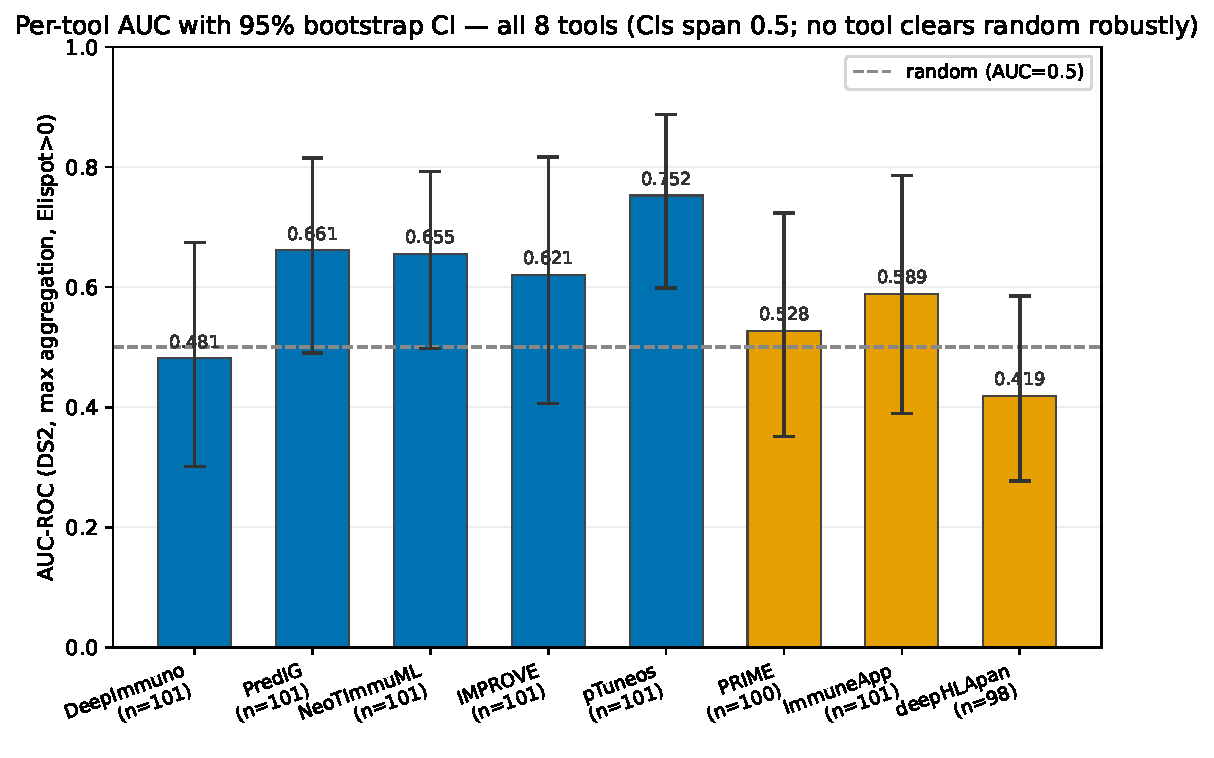
\includegraphics[width=\linewidth]{figures/fig6_auc_comparison.pdf}
\caption{AUC-ROC for the eight tools at the three thresholds (SFC $>0$, $>10$,
$>$ median) under best-binder aggregation. New-wave tools are highlighted.}
\label{fig:auc}
\end{figure}

\begin{figure}[t]
\centering
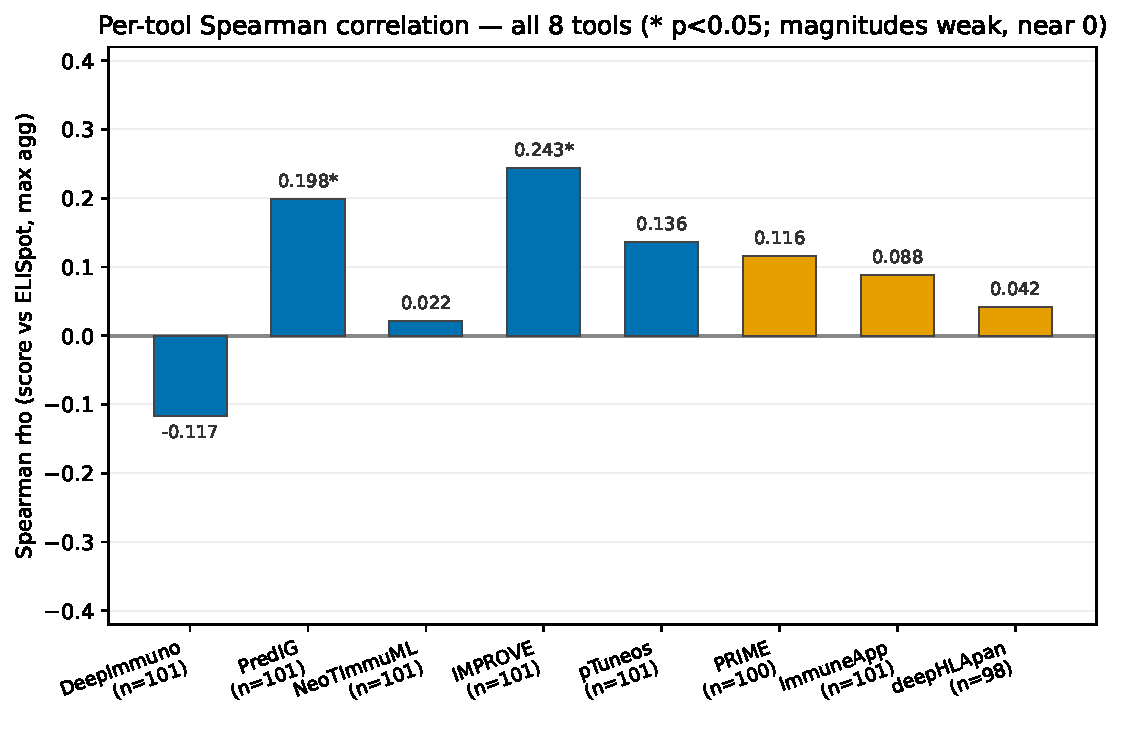
\includegraphics[width=\linewidth]{figures/fig7_spearman.pdf}
\caption{Spearman correlation between tool score and ELISpot SFC under
best-binder aggregation; $^{*}$ marks $p < 0.05$. All point estimates satisfy
$|\rho| < 0.33$.}
\label{fig:spearman}
\end{figure}

\subsection{Aggregation, threshold sensitivity, and bootstrap uncertainty}
\label{sec:res-sensitivity}

The point-estimate ordering in Table~\ref{tab:main} is fragile in two distinct
ways, and we report both so that the leading position is not mistaken for a
statistically established advantage.

\paragraph{Sensitivity to aggregation and threshold.} The leading AUC is not
stable across operating points. pTuneos rises to AUC $= 0.7813$ under mean
aggregation at the SFC $>0$ threshold, but the same tool falls to
$\approx 0.46$---below chance---when the threshold is moved to the cohort median,
indicating that its apparent discrimination is concentrated at one operating
point rather than reflecting a robust capability. Aggregation choice alone can
move a tool materially: ImmuneApp improves from AUC $= 0.5889$ under maximum
aggregation to $0.6444$ under mean aggregation at the same SFC $>0$ threshold
(a shift of $+0.055$), confirming that its score is sensitive to how the
per-window, per-allele values are summarized. These observations are exactly why
the headline comparison is locked to a single aggregation--threshold combination
(Section~\ref{sec:fairness}); allowing each tool its own best-of-nine operating
point (\emph{selection-on-max}) would award different tools different conventions
and is reported only descriptively. Under such per-tool best-of-nine selection,
the highest \emph{significant} magnitude correlations belong to IMPROVE
(top3mean aggregation, $\rho = 0.3202$, $p = 0.0011$) and PredIG (mean
aggregation, $\rho = 0.2797$, $p = 0.0046$); we present these as descriptive
upper envelopes per tool and not as a cross-tool ranking, since the operating
points differ.

\paragraph{Bootstrap uncertainty.} A $2000$-replicate bootstrap shows that the
leading AUC carries a wide confidence interval: pTuneos has AUC $= 0.7525$ with a
$95\%$ CI of $[0.598, 0.888]$. The per-tool intervals are wide and broadly
overlapping---for example PredIG $[0.490, 0.815]$ and NeoTImmuML$^\star$
$[0.498, 0.792]$ both overlap the pTuneos interval substantially. A paired
bootstrap of the between-tool AUC differences confirms that pTuneos's lead over
its nearest competitors is not significant: $\Delta\mathrm{AUC}$ against PredIG is
$0.0914$ with a $95\%$ CI of $[-0.145, 0.310]$, and against ImmuneApp is $0.1636$
with a CI of $[-0.093, 0.414]$, both spanning zero. We therefore describe pTuneos
as ranking first by point estimate, and we explicitly do not claim a single best
or strongest tool at the top of the panel. The same paired bootstrap does,
however, separate the upper group from the lower half: pTuneos's advantage reaches
significance against IMPROVE ($\Delta\mathrm{AUC} = 0.1318$, CI $[0.006, 0.287]$),
PRIME ($0.2283$, CI $[0.044, 0.434]$), and deepHLApan ($0.3517$, CI
$[0.040, 0.589]$), whose intervals exclude zero. This pattern is consistent with a
weak but real separation between an upper and a lower group of tools rather than a
single dominant predictor. The driver of the residual uncertainty is the cohort
size: DS2 contains $101$ peptides with only $11$ negatives, which is too small to
resolve AUC differences of the magnitude seen at the top of the table.

\begin{table}[t]
\centering
\caption{Bootstrap uncertainty on AUC-ROC under the locked configuration
($2000$ replicates). The leading tool's confidence interval is wide, and the
paired $\Delta\mathrm{AUC}$ intervals against its two nearest competitors
include zero (top block), so we do not claim a single best tool. The same paired
bootstrap does separate pTuneos from the lower half of the panel (bottom block),
whose intervals exclude zero.}
\label{tab:bootstrap}
\begin{tabular}{lcc}
\toprule
Comparison & $\Delta\mathrm{AUC}$ (point) & $95\%$ CI \\
\midrule
pTuneos AUC (absolute)                & $0.7525$ & $[0.598, 0.888]$ \\
\midrule
pTuneos $-$ PredIG                    & $0.0914$ & $[-0.145, 0.310]$ \\
pTuneos $-$ ImmuneApp                 & $0.1636$ & $[-0.093, 0.414]$ \\
\midrule
pTuneos $-$ IMPROVE                   & $0.1318$ & $[0.006, 0.287]$ \\
pTuneos $-$ PRIME                     & $0.2283$ & $[0.044, 0.434]$ \\
pTuneos $-$ deepHLApan                & $0.3517$ & $[0.040, 0.589]$ \\
\bottomrule
\end{tabular}

\vspace{2pt}
{\footnotesize A paired comparison against NeoTImmuML$^\star$ was not computed;
its overlapping per-tool interval ($[0.498, 0.792]$) is reported in the text.}
\end{table}

\begin{figure}[t]
\centering
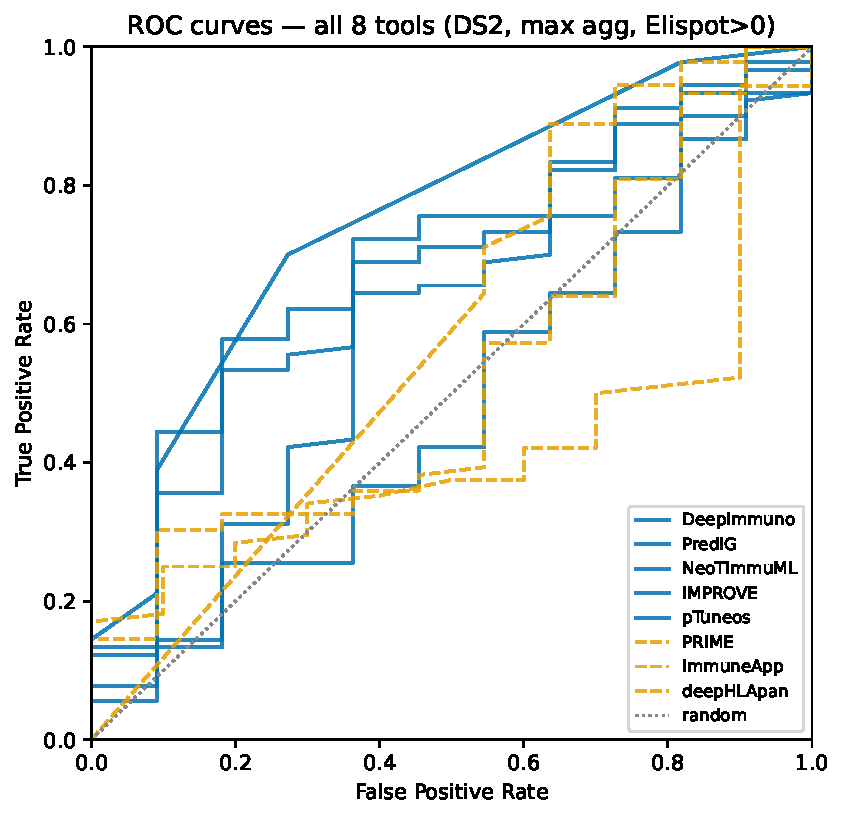
\includegraphics[width=\linewidth]{figures/fig8_roc_curves.pdf}
\caption{ROC curves for the eight tools at the SFC $>0$ threshold under
best-binder aggregation. New-wave tools are shown with dashed lines.}
\label{fig:roc}
\end{figure}

\subsection{Per-patient evaluation reorders the panel}
\label{sec:res-perpatient}

The global correlations in Table~\ref{tab:main} pool all peptides across patients
and can mask a tool's ability to rank candidates \emph{within} an individual
patient. Recomputing the magnitude correlation under the per-patient protocol of
Section~\ref{sec:perpatient}---a Fisher-$z$ weighted mean of the per-patient
$\rho_i$, with the median reported as a robust co-primary estimate---changes both
the magnitude and the ordering of the results (Table~\ref{tab:perpatient}).

% XXX_HLA-FIX[投稿前必更新]: 以下 per-patient 头条数字(PRIME 0.253/0.386, deepHLApan 0.261/0.402 等)均在含 P101/P102 等位伪迹的 9 患者上计算，修复后必变、相对排序可能动。待 Phase B 正确等位重推理后用 corrected 数据重算。数字暂不动=拍板点(P102 等位待袁老师确认)，见文件头 TODO + 04_LOG Entry HLA-FIX。
The most striking shifts occur for tools that are near the noise floor globally.
PRIME moves from a global $\rho = 0.1163$ to a per-patient Fisher-$z$ weighted
estimate of $0.253$ and a median of $0.386$, a change of $+0.270$ in the median
relative to the global value. Crucially, this jump is not an artifact of peptide
length: under best-binder aggregation PRIME's pooled peptide-level scores are
essentially uncorrelated with the number of constituent sub-peptides
($\rho \approx 0.13$), so the per-patient gain reflects a genuine within-patient
reordering rather than a length proxy. IMPROVE shows the same clean pattern, moving
from a global $\rho = 0.2434$ to a Fisher-$z$ estimate of $0.250$ and a median of
$0.268$, and its scores are likewise length-insensitive ($\rho \approx 0.12$).
DeepImmuno, which carries a negative global point estimate ($-0.1168$), moves to a
Fisher-$z$ estimate of $0.0127$ and a median of $-0.05$, i.e.\ toward zero but
without a meaningful within-patient signal. This
reordering shows that the global Spearman is not merely a noisy version of the
per-patient estimate; for some tools it has the wrong sign or magnitude because
it conflates between-patient and within-patient variation.

A large per-patient jump must not, however, be read uncritically as within-patient
capability, because the underlying peptide-level scores can themselves be
confounded. deepHLApan is the cautionary case. Its global $\rho = 0.0415$ rises to
a per-patient Fisher-$z$ estimate of $0.261$ and a median of $0.402$---numerically
the largest shift in the panel---but under best-binder aggregation its pooled
scores are strongly correlated with peptide length, as captured by the number of
constituent sub-peptides ($\rho \approx 0.57$), well above the $\rho = 0.5$ level
at which we treat an aggregation as count-confounded. Re-pooling deepHLApan with
length-insensitive operators---\texttt{mean} or the geometric mean, whose own
correlation with peptide length is negligible ($\rho \approx 0.08$)---collapses its
correlation with immunogenicity to $\approx 0$. The per-patient jump for deepHLApan
therefore largely tracks peptide length rather than within-patient immunogenicity
ranking, and we report it as a cautionary example---per-patient correlation does
not by itself remove aggregation-level confounds
(Section~\ref{sec:harmonization})---rather than as evidence of ranking ability.

Underneath these aggregates is substantial individual heterogeneity that the
global number averages away. The core methodological finding is that pooling can
cancel a genuine within-patient signal: PRIME's clean $+0.270$ median jump shows
that a tool dismissed as near-noise globally can in fact order candidates within
individual patients, a structure the cohort-wide Spearman conceals. The underlying
per-patient coefficients are also widely dispersed; for deepHLApan they range from
$-0.43$ to $+0.81$ with a standard deviation of $0.46$, so the tool appears to rank
candidates well within some patients and inversely within others. As noted above,
however, deepHLApan's positive tail is inflated by the peptide-length confound, so
we read this spread as descriptive only. This dispersion also bounds how strongly
we can state any per-patient claim. With only $K = 9$ patients and small
per-patient sample sizes ($n_i = 5$--$16$), the per-patient aggregates carry wide
confidence intervals; we therefore anchor the claim on the Fisher-$z$ weighted mean
and the median together, treat the dispersion as descriptive, and flag the
small-sample caveat explicitly rather than ranking tools by these estimates.

\begin{table}[t]
\centering
\caption{Global versus per-patient magnitude correlation under best-binder
aggregation. Per-patient estimates aggregate the within-patient $\rho_i$ over
$K = 9$ patients ($n_i = 5$--$16$); the Fisher-$z$ weighted mean and the median
are co-primary. $\Delta$ is the median minus the global value. The reordering is
largest for tools near the global noise floor; PRIME is a clean exemplar, whereas
deepHLApan ($^{\dagger}$) is count-confounded under best-binder aggregation (see
note). Estimates carry wide confidence intervals owing to small $K$ and $n_i$ and
are not used to rank tools.}
\label{tab:perpatient}
\begin{tabular}{lcccc}
\toprule
Tool & Global $\rho$ & Fisher-$z$ mean & Median $\tilde{\rho}$ & $\Delta$ (med.\ $-$ glob.) \\
\midrule
PRIME                  & $0.1163$  & $0.253$  & $0.386$  & $+0.270$ \\
deepHLApan$^{\dagger}$ & $0.0415$  & $0.261$  & $0.402$  & $+0.360$ \\
DeepImmuno             & $-0.1168$ & $0.0127$ & $-0.05$  & $+0.067$ \\
\bottomrule
\end{tabular}

\vspace{2pt}
{\footnotesize $^{\dagger}$deepHLApan's per-patient jump is count-confounded under
best-binder aggregation: its pooled scores correlate with peptide length
($\rho \approx 0.57$) and the signal collapses to $\approx 0$ under
length-insensitive pooling, so this row is a cautionary case rather than evidence
of within-patient ranking ability. Per-patient aggregates (Fisher-$z$ weighted
mean; median) for the remaining tools: IMPROVE $0.250$; $0.268$, PredIG $0.230$;
$0.291$, pTuneos $0.170$; $0.159$, NeoTImmuML$^\star$ $0.033$; $0.058$, ImmuneApp
$0.173$; $0.187$. IMPROVE and PredIG remain among the top of the panel under both
the global and the per-patient view.}
\end{table}

\begin{figure}[t]
\centering
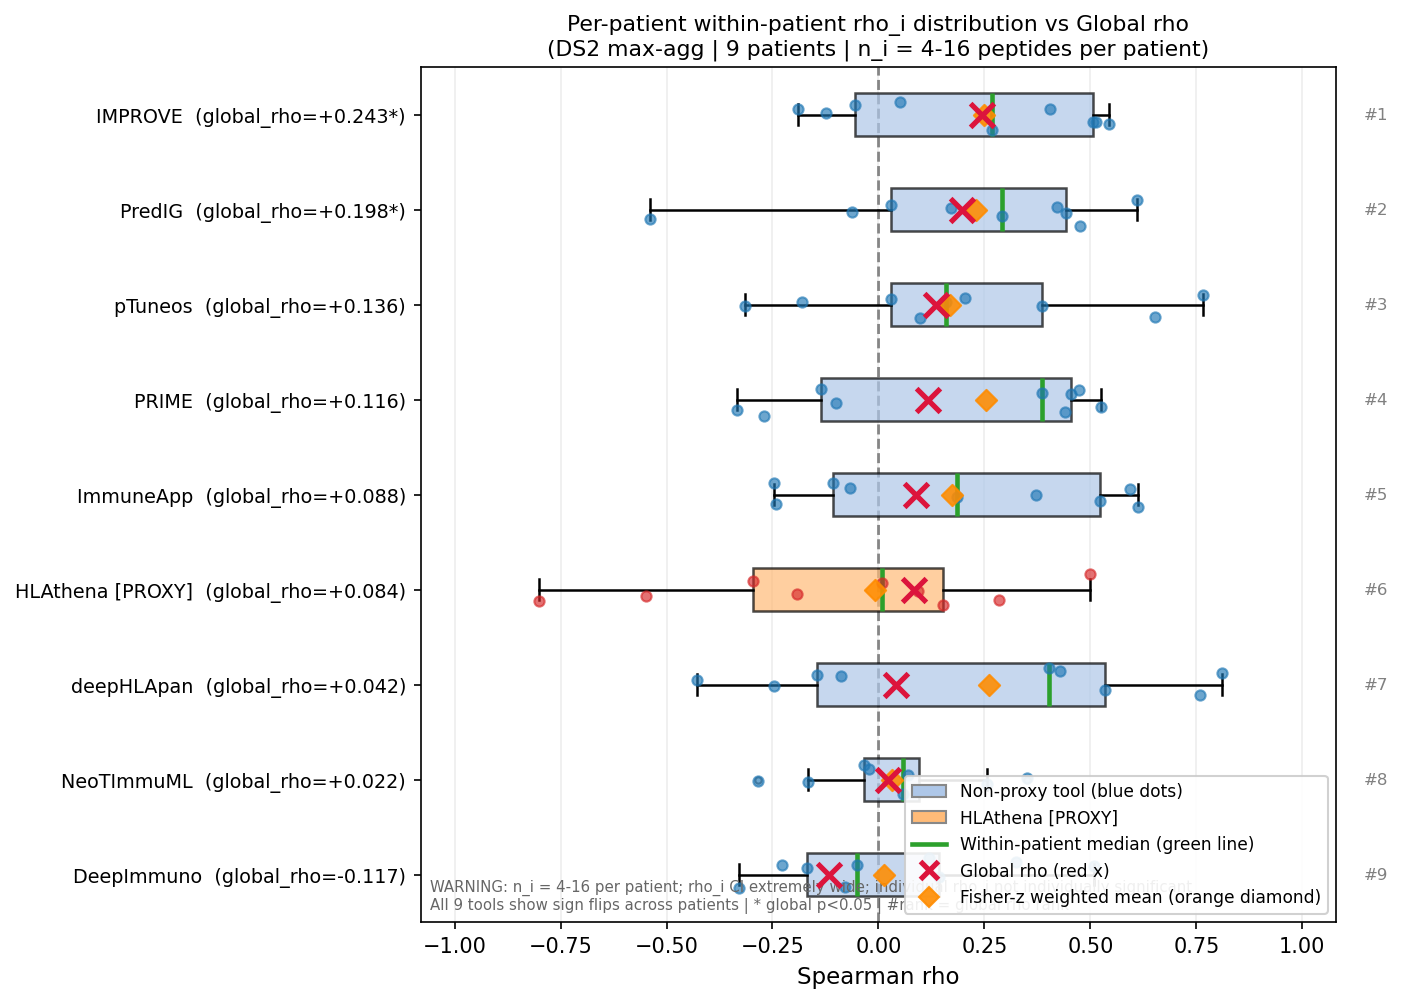
\includegraphics[width=\linewidth]{figures/fig9_perpatient.png}
% NOTE(coder): a dedicated per-patient rho_i strip/box plot with global vs Fisher-z/median
% overlay would sharpen this panel; current figure is the per-patient factor plot.
\caption{Distribution of per-patient $\rho_i$ for each tool, with the global
correlation and the Fisher-$z$/median aggregates overlaid. PRIME is a clean
exemplar of the heterogeneity hidden by the pooled estimate: a near-noise global
correlation ($\rho = 0.1163$) resolves into a positive within-patient median
($0.386$) with no peptide-length confound. The very wide spread for deepHLApan
($\rho_i \in [-0.43, +0.81]$, $\mathrm{std} = 0.46$) is shown for contrast, but
part of its positive tail reflects the peptide-length confound discussed in the
text and should not be read as within-patient ranking ability.}
\label{fig:perpatient}
\end{figure}

\subsection{Presentation proxy as a near-random anchor}
\label{sec:res-proxy}

Finally, the presentation proxy behaves as expected for a quantity that captures
peptide display rather than functional immunogenicity. HLAthena attains an
AUC of $\approx 0.51$ on the binary discrimination task---essentially random---and
its per-patient magnitude correlation is $\approx 0$. Because HLAthena scores
binding/presentation rather than T-cell activation, this near-random result is not
a failure of the proxy but a calibration anchor: it empirically separates the
three quantities at issue in this benchmark, namely presentation, immunogenicity
(positive/negative recognition), and magnitude (response strength). Presentation
is a necessary precondition for recognition, but on this cohort it carries no
information about either the binary recognition call or the continuous magnitude,
which is consistent with treating magnitude prediction as a distinct and
currently unmet capability (Section~\ref{sec:discussion}).

% TODO[HLA-FIX 2026-06-27]: PredIG 全局显著性已失效(max-pool rho 0.198->0.104 p=0.343 ns; mean-agg 0.280->0.188 p=0.084 ns)，剔污染患者 P101/P102 后不存活；IMPROVE 仍稳健显著(0.226 p=0.037)，TSCAPE 翻为显著负(-0.230 p=0.033)，deepHLApan 另有 merge bug 双重不可信；per-patient 头条数字(PRIME/deepHLApan)待 Phase B 正确等位重推理后更新。正文数字暂不动(投稿=拍板点 + P102 等位待袁老师确认)。详见 04_LOG Entry HLA-FIX。
\section{Discussion}
\label{sec:discussion}

\subsection{Existing tools do not quantify response magnitude}
\label{sec:disc-gap}

The benchmark gives a direct, empirical answer to the question that motivated it:
when the scores of current immunogenicity predictors are repurposed as continuous
estimators of T-cell response magnitude, they track it poorly. Across the eight
tools, every absolute Spearman correlation with ELISpot magnitude falls below
$0.33$, and only IMPROVE and PredIG reach significance, and then only under
% XXX_HLA-FIX[投稿前必改]: 修复后此句不再成立——剔 P101/P102 后 PredIG 全局显著性失效(p=0.343 ns)，"only IMPROVE and PredIG" 须改为 "only IMPROVE"。数字暂不动=拍板点，见文件头 TODO + 04_LOG Entry HLA-FIX。
particular aggregation choices (Section~\ref{sec:results}). This is consistent
with, and quantifies, the gap we identified in the literature survey: no surveyed
method is designed to regress magnitude, and several discard the graded signal
their own training data contain. IMPROVE and PredIG are trained on data that
distinguish graded response levels but are binarized before use
\cite{IMPROVE2024,PredIG2025}, and other tools collapse graded labels into a
single recognition class. The benchmark therefore turns a documentary
observation---that the field reports binary calls---into a measured one: even the
best-performing current scores explain only a small fraction of the variance in
how strongly patients respond. We read the convergence of the survey evidence and
the empirical correlations as showing that the magnitude gap is real rather than
an artifact of how individual papers report their results.

A weak correlation, however, is not automatically a deficiency to be engineered
away. The same result is compatible with two readings---tools that could do
better but were never asked to, or a target that is intrinsically hard to predict
from the available inputs---and the next subsection argues that both readings hold
simultaneously.

\subsection{A biological ceiling bounds what sequence-level prediction can achieve}
\label{sec:disc-ceiling}

There is a structural reason to expect that magnitude prediction from peptide and
allele alone is bounded well short of perfect. The magnitude of a polyclonal
T-cell response is, to a first approximation, the product of a recruitment-and-
expansion chain whose leading term is the number of naive precursor T cells
specific for the epitope; in mouse models, naive precursor frequency is reported
to be a major determinant of the magnitude of the elicited
response~\cite{Jenkins2012,Moon2007}. The quantitative form of this dependence in
human neoantigen-specific CD8 responses has not been established and the
extrapolation across species and T-cell subset is uncertain, but the qualitative
direction---that a host-specific, sequence-invisible quantity gates response
size---is expected to carry over. That quantity is a property of the
host's T-cell repertoire and thymic selection history, varies substantially
across donors for the same peptide and allele, and is in principle unobservable
from a peptide-and-HLA input. Writing the explainable variance as a ratio,
\begin{equation}
  \rho_{\max}^2 \;\le\; \frac{\operatorname{Var}\!\big(\mathbb{E}[Y \mid X]\big)}
                              {\operatorname{Var}(Y)},
  \label{eq:ceiling}
\end{equation}
where $Y$ is the measured magnitude and $X$ the peptide-and-allele input, the
donor-specific precursor and repertoire terms sit in the numerator's complement
and cannot be recovered no matter how much sequence data are supplied. A
first-order analysis along these lines places the attainable rank correlation at
roughly $\rho_{\max}\approx 0.4$ to $0.6$; we present this figure as a positional
estimate rather than a measured bound, since it rests on biological variance
parameters we did not measure directly. Read against this ceiling, the best
magnitude correlation under the locked primary protocol (IMPROVE,
$\rho = 0.2434$) already reaches roughly half of the lower end of the plausible
maximum; even the per-tool upper envelope obtained by allowing each tool its own
best-of-nine operating point---a descriptive figure we do not treat as a fair
ranking (Section~\ref{sec:fairness})---tops out near $\rho\approx 0.32$ for IMPROVE,
on the order of half to two-thirds of the ceiling. Either way the headroom for
pure sequence-level magnitude regression appears modest rather than large.

We take a deliberate position on what this implies for tool design. If the
ceiling on pure peptide-and-HLA inputs is genuinely in the middle of the range,
then the value of a continuous-magnitude model should not be advertised as
high-precision regression. It should instead be framed as recovering
ranking-relevant signal for clinical top-$K$ prioritization---where only a handful
of peptides can be synthesized into a vaccine and the quality of the ordering is
what matters---which binary tools discard by construction. Breaking past the
ceiling would require feeding donor-specific information (HLA typing, T-cell
receptor repertoire, or precursor estimates) rather than a more elaborate
sequence model.

\subsection{Per-patient evaluation should be the default}
\label{sec:disc-perpatient}

A methodological lesson generalizes beyond the tools we ranked. Pooling all
peptides across patients into a single global correlation can hide a tool's
ability to order candidates \emph{within} an individual patient, which is the
quantity that actually governs vaccine selection. Several tools whose pooled
global correlation is indistinguishable from noise show within-patient ranking
ability in a subset of patients---alongside substantial dispersion---once the
correlation is computed per patient and then summarized: PRIME moves from a global
Spearman of $0.116$ to a per-patient median coefficient of $0.386$ (and a
Fisher-$z$ weighted mean of $0.253$), and because its best-binder scores are
essentially uncorrelated with peptide length, this gain reflects a genuine
within-patient reordering rather than a length artifact
(Section~\ref{sec:results}). A per-patient jump must nonetheless be checked against
aggregation-level confounds before it is read as capability: deepHLApan shows the
numerically largest shift (global $0.042$ to a per-patient median of $0.402$), but
under best-binder aggregation its pooled scores correlate with peptide length
($\rho \approx 0.57$) and the signal collapses to $\approx 0$ under
length-insensitive pooling, so we treat its jump as a cautionary case rather than
as evidence of within-patient ranking ability. Because of the wide individual
heterogeneity ($\rho_i$ spanning roughly $-0.43$ to $+0.81$ for the most dispersed
tools) we read the per-patient aggregates as descriptive summaries of central
tendency rather than as estimates of a single common correlation, and we anchor the
qualitative claim on the median together with the reported spread. The global metric is not wrong, but it answers a
different question---can a single score threshold separate responders across an
entire cohort---than the clinically relevant one. We therefore recommend that
benchmarks of magnitude or ranking ability compute the metric per patient before
aggregating, mirroring the cohort-level paradigm of the clinical neoantigen
literature \cite{TESLA2020,Muller2023}, and report the across-patient spread
rather than a single pooled number.

\subsection{Limitations}
\label{sec:disc-limits}

Several limitations bound our conclusions and we state them plainly. First, the
primary cohort is small and imbalanced: DS2 contains $101$ peptides with only
$11$ negatives at the SFC $>0$ threshold and $K=9$ patients with $5$ to $16$
peptides each, so every per-patient aggregate carries a wide confidence interval
and the per-patient point estimates should not be over-read. We report bootstrap
and Fisher-$z$ intervals throughout for this reason, and we draw conclusions from
the consistency of the pattern across aggregation choices rather than from any
single coefficient. Second, our results rest on a single benchmark cohort;
external replication on independent ELISpot cohorts is needed before the ranking
behavior can be generalized. Third, several tools were trained on IEDB-derived
data that may overlap with the benchmark peptides, which would bias those tools
optimistically; we note that this works \emph{against} our central claim rather
than for it, since even with any such advantage no tool achieves a strong
magnitude correlation. Fourth, three tools are evaluated in non-canonical
configurations that we carry through every table: NeoTImmuML is a model retrained
by us because official weights are unavailable (denoted NeoTImmuML$^\star$),
pTuneos is run through its Pre\&RecNeo sub-model, and IMPROVE is run with its
expression feature degraded; our statements about these tools refer to the
configuration actually evaluated, not necessarily to the original published
models. Because a degraded or retrained configuration can only lower a tool's
apparent performance relative to its full published form, our central claim---that
current tools do not recover response magnitude---is, for these three tools, a
conservative statement rather than an upper bound on what the original models could
achieve; it remains directly supported by the five tools evaluated in their
intended configurations. Finally, the expanding second wave of predictors and the tools governed by
restrictive academic data-use terms are integrated into the pipeline but their
results are withheld from the main conclusions, which do not depend on them.

\subsection{Future work}
\label{sec:disc-future}

The natural sequel to this benchmark is a predictor built to occupy the L4 rung
directly: a model that regresses continuous response magnitude against ELISpot
SFC rather than emitting a binary call. The benchmark supports such an effort in
two concrete ways. It establishes that the gap is real and currently unfilled,
which is the empirical justification for attempting it, and it provides a
reproducible evaluation protocol---harmonized inputs, the best-binder aggregation,
the per-patient analysis, and the bootstrap intervals---against which any
candidate magnitude predictor can be measured on equal terms. Consistent with the
ceiling argued in Section~\ref{sec:disc-ceiling}, we expect the realistic payoff
of such a model to lie in improved clinical top-$K$ ranking rather than in
high-accuracy regression, and we regard the incorporation of donor-specific
information as the most promising, if speculative, route to pushing past the
sequence-level ceiling.

\section{Conclusion}
\label{sec:conclusion}

We set out to ask whether today's neoantigen immunogenicity tools can quantify the
\emph{magnitude} of a T-cell response, and to do so under a controlled,
apples-to-apples protocol rather than across incomparable papers. Three
conclusions follow. First, under a unified seven-step harmonization protocol,
existing tools do not quantify magnitude: across eight immunogenicity predictors
and one presentation proxy, every absolute Spearman correlation with the
continuous ELISpot readout falls below $0.33$, binary-discrimination differences
have broadly overlapping bootstrap intervals that shift with aggregation and
threshold, and no single tool is statistically distinguishable as best. Second, a
per-patient evaluation protocol recovers within-patient ranking ability that the
default global correlation conceals, exposing substantial individual variation
and arguing that benchmarks in this area should compute their metrics per patient
before aggregating. Third, response magnitude is a systematically overlooked gap,
but one bounded by a genuine biological ceiling: because the leading driver of
magnitude is a donor-specific precursor frequency invisible to peptide-and-allele
inputs, the explainable variance is structurally capped, and the value of
continuous prediction is best framed as ranking gain for clinical
top-$K$ selection rather than as high-precision regression.

Taken together, these findings reframe magnitude prediction as an open and
worthwhile---yet bounded---problem, and supply a reproducible benchmark and
per-patient protocol against which future continuous-magnitude predictors can be
measured. We hope the benchmark serves both as an honest baseline for what current
tools achieve and as a measuring stick for the quantitative immunogenicity models
that this gap invites.


% 数据/代码可用性 + DTU pending 声明
\section*{Data and Code Availability}
\paragraph{Data.} The benchmark uses functional T-cell readouts measured by
interferon-$\gamma$ ELISpot on neoantigen candidates. All peptide sequences,
HLA assignments, and ELISpot spot-forming-count values were de-identified before
analysis and carry no patient-identifying information. To preserve the
double-blind review process, the originating cohort and any contributing
institutions are withheld from this version and will be named, with the
appropriate accession or controlled-access details, in the camera-ready version.

\paragraph{Code.} The harmonization pipeline, the per-tool scoring wrappers, the
per-patient evaluation protocol, and the analysis scripts that produce every
table and figure in this paper are organized for reproducible re-execution and
will be released in a public repository upon publication. To support peer review,
an anonymized snapshot of the code together with the harmonized, de-identified
derived score tables (per tool, per peptide) and the per-patient correlation
outputs underlying every table and figure are made available to reviewers and
editors, so that all reported metrics can be regenerated end to end without access
to any patient-identifying data.

\paragraph{Restricted tools and pending results.} A subset of predictors is
distributed under academic data-use agreements that restrict redistribution and
the publication of derived numbers---these include the netMHCpan, netMHCstabpan,
and NetTepi families and the related expansion-wave tools integrated into the
pipeline. The results for these tools are \emph{not} included in the main
conclusions of this paper and are marked \pendingDTU\ throughout. They will be
reported only after the required written data-use consent has been obtained, and
the full provenance and licensing status of every tool is tracked separately
(see the accompanying provenance record). The headline claims of this paper do
not depend on any restricted tool.


\bibliographystyle{unsrtnat}
\bibliography{refs}

\end{document}
